\chapter{低驱动电压硅基混合集成电光吸收调制器}
基于QCSE效应的电吸收光调制器具有高速,低能耗,高消光比和小尺寸的特别点\cite{tang2012energy, fukano2006very}。因此电吸收光调制器被广泛应用于光通信领域。另外,电吸收调制器具有双工作模,还可以被用于高速的光探测器\cite{welstand1996dual}。基于这个特性,研究人员实现了光电振荡器(Optoelectronic Oscillators, OEO)\cite{zhou2014compact}。我们最近也实现了单片集成的光收发器\cite{chen2016wavelength}。最近,由于硅光子和晶体管在统一的半导体工艺线上制作,这给复杂的光电集成系统,比如集成光子微波系统\cite{Marpaung2013integrated}和芯片间的光互联系统\cite{sun2015single},带来了希望。基于硅和III-V的键合技术,已经实现硅基混合集成III-V光调制器\cite{kuo2008high,tang201150,tang2012over,tang2012energy,chen2011forty,Srinivasan2012micro,fu20155}。不过,硅基光芯片中,低能耗是十分重要的指标。又因为电吸收光调制器的驱动电压与能耗成平方关系,见公式\ref{Equ:EC}。因此,硅基光芯片中低驱动电压的光调制器十分重要。另外,如果电吸收光调制器能够直接被来自逻辑电路的低电压信号驱动,那么消耗于电的放大器的能量也会被省下来。最近,研究人员们在纯硅上展示了100~mV一下的硅基光调制器,见表格\ref{sil_mod}。然而,这些硅的调制器都是基于光的谐振腔结构,见图\ref{fig_mod_opt_type}(a)所示,它们对工艺的要求十分苛刻,并且还不能用于光探测器。对于传统的基于QCSE的电吸收光调制器,降低驱动电压的同时保持同样的尺寸和插入损耗十分困难。尽管研究人员利用复杂的基于慢光效应的布拉格波导\cite{gulow-voltage2013},降低了电吸收光调制器的驱动电压,但是这种结构的光调制器不仅无法和硅光子器件集成也无法将驱动电压降低到硅调制器层次。因此,我们需要寻找一种新的思路实现的驱动电压的光调制器。

本章概述了基于能带填充效应的新型低驱动电吸收光调制器,首先介绍了低驱动电压电吸收调制器的理论原理。接着阐述了设计和和仿真结果。然后,详细接收了制作调制器的步骤。最后,在搭建的高速光调制器测试平台上,对低驱动电压光调制器的性能进行了测试。
\section{低驱动电压光调制器的原理}
\begin{figure}[htb]
	\centering
	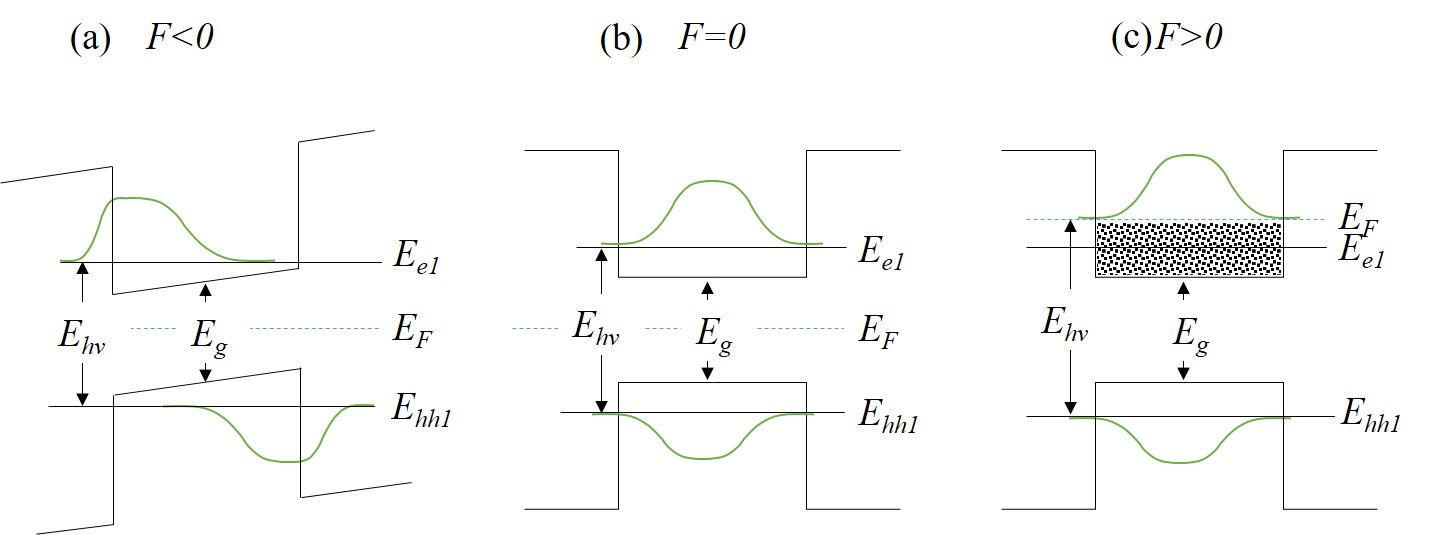
\includegraphics[width=14cm]{./Pictures/fig_ch4_bandfilling_diag.jpg}
	\caption{ 量子阱的能带和波函数的示意图(a)有外界反向电场下;(b)在外界无电场的时候;(b)在外界正向电子子注入的时候}
	\label{fig_ch4_band_lineup}
\end{figure}
调制掺杂中的多量子阱 (Modulation-doped Multiple Quantum-wells) 中的能带填充效应在80年代已经被深入研究\cite{livescu1988free}。能带填充效应与QCSE效应的原理示意图见图\ref{fig_ch4_band_lineup}。当正向电子注入多量子阱中势阱的导带时,相应的电子准费米能级就提高。当电子的准费米能级高过导带中最低的能级时,即最低的能级被二维电子气体填充慢时,导致了原本激子吸收峰对应的光子无法被吸收,因此其产生的电子无法跃迁到最低的能级处。这意味着只有更高能量的光子才会被吸收,使产生电子跃迁到费米能级处。可以预测随着注入电子浓度的增加,使电子的准费米能级的逐渐升高,导致了激子吸收峰的蓝移。除此之外,根据公式\ref{Equ:excitonabs}所示,激子吸收峰的强度与电子空穴波函数的重叠积分成平方关系。。基于QCSE效应,外加的电场会使能带结构倾斜,从而电子空穴的重叠积分减弱,如图\ref{fig_ch4_band_lineup}(a)所示,导致激子吸收峰随着外界电场的增强而减弱,见图\ref{fig_ch2_te_abs}。而基于能带填充效应,由于能带结构并不会发生明显变化(只会由于电子间的多体效应导致能带结构发生微弱的形变\cite{livescu1988free}),电子和载流子的波函数与无外界电场几乎相同,如图\ref{fig_ch4_band_lineup}(c)所示,因此激子吸收峰的强度随着电子浓度的增加而将保持一致。这为实现低驱动电压的电吸收光调制器提供了条件。

激子吸收峰对应光子能量的漂移量$\Delta E$与电子准费米能级$E_F$的关系如下式所示\cite{livescu1988free}:
\begin{equation}
\label{Equ:DEEF}
\Delta E = (1+m_e/m_h)E_F,
\end{equation}
其中$m_e$和$m_h$分别是电子和空穴的等效质量。当$E_F$远大于导带中最低的能级$E_1$时,电子的准费米能级和量子阱中载流子浓度成线性关系,见公式\ref{Equ:E1EF}\cite{coldren1995diode}。
\begin{equation}
\label{Equ:E1EF}
E_F = \pi\hbar^2d_xN/m_e+E_1,
\end{equation}
其中$d_x$是多量子阱中所有势阱的宽度\textsl{}。我们可以通过控制偏置电压,调节注入电流,从而调节量子阱区域的电子浓度。电流与载流子浓度的关系见公式\ref{Equ:VN}。
\begin{equation}
\label{Equ:VN}
N = \frac{\tau\eta I}{qV}
\end{equation}
其中,$\tau$是载流子寿命,$\eta$是载流子注入效率,I是注入电流,V是调制器有源区体积,q是电子的基本电荷。因此,利用能带填充效应,多量子阱的激子吸收峰的位置就可以通过偏置电压来控制。利用调制掺杂的多量子阱中的能带填充效应,已经被应用于100~mV驱动电压的Q调制器的激光器\cite{kalinovsky1993free}。而我们在此展示的低驱动电压的电吸收光调制器是首个基于能带填充效应的光调制器。

\section{调制器的设计与仿真}
考虑到电子束光刻制作III-V和硅耦合结构工艺困难。我们设计的低驱动电压的硅基混合集成电吸收调制器将采用普通的接触式光刻工艺制作,并且波导加工将采用纯湿法腐蚀,降低工艺成本。因此,我们将采用蘑菇型的波导结构。波导截面结构示意图,如图\ref{}所示。硅波导的结构是380~nm厚,刻蚀深度160~nm的脊型波导。并且表面利用SiO\SB{2}进行平坦化。接下来是利用DVS-BCB和SiO\SB{2}的键合层。在往上是III-V结构,与图\ref{fig_ch2_banddiagram}相同。具体结构的组分如表\ref{epi_material},各个组分的材料参数,比如折射率等,见表\ref{epi_structure}。
{
	\begin{table}[htb]
		\zihao{5}
		\caption{III-V 波导的材料参数。$\lambda_{ex}$:激子吸收峰波长}
		\label{epi_material}
		\centering
		\begin{tabular}[t]{llll}
			\hline
			名称 & 材料组分 & 掺杂浓度 (cm\SP{-3}) & 厚度 \\
			\hline
			p-contact &In\SB{0.53}Ga{0.47}As& p-1.5$\times$10\SP{19}& 0.1$\mu m$  \\ 
			\hline
			p-cladding  & InP & p-2$\times$10\SP{18} to p-1$\times$10\SP{18} &1.5 $\mu m$ \\
			\hline
			SCH & In\SB{0.52}Al\SB{0.16}Ga\SB{0.32}As& - &0.15 \\
			\hline
			\multirow{2}{*}{\tabincell{l}{MQW \\ ($\lambda_{ex} = 1560~nm$)}}
			& Well:~In\SB{0.65}Al\SB{0.09}Ga\SB{0.26}As,(10$\times$) & -& 110~nm\\ 
			\cline{2-4} 
			&Barrier:~In\SB{0.42}Al\SB{0.17}Ga\SB{0.39}As,(11$\times$) &-& 70~nm\\
			\hline
			SCH & In\SB{0.52}Al\SB{0.16}Ga\SB{0.32}As& - & 0.1 $\mu m$\\
			\hline
			n-contact & InP& n-3$\times$10\SP{18} & 0.15 $\mu m$ \\
			\hline
		\end{tabular}
	\end{table}
}
\section{混合集成调制器的制作}
\section{性能测试}
